\chapter{RESULTADOS}
\label{cap:resultados}

Este capítulo presenta los resultados experimentales de GBMARL siguiendo el orden de construcción del marco: la calibración del simulador (Sección~\ref{sec:res-calibracion}), la validación del entorno y la convergencia del aprendizaje (Sección~\ref{sec:res-aprendizaje}), la comparación frente a las líneas base con la métrica auditada (Sección~\ref{sec:res-comparacion}), el mecanismo de la política aprendida (Sección~\ref{sec:res-mecanismo}), la ablación del crítico centralizado (Sección~\ref{sec:res-ablacion}), el análisis de sensibilidad (Sección~\ref{sec:res-sensibilidad}) y la robustez adversarial mediante explotabilidad (Sección~\ref{sec:res-explotabilidad}). La interpretación de estos hallazgos y sus implicaciones se desarrollan en el capítulo siguiente.

\textbf{Nota de estado.} Las cifras de esta revisión se distinguen entre resultados históricos y la auditoría calibrada del 8 de septiembre de 2026. La auditoría usa DepMap Public 26Q1, GDSC2 release 8.5 y la huella de parámetros \texttt{1fd8464abb97}; las tablas históricas que aún no fueron reejecutadas con esa huella se mantienen únicamente como referencia y no deben combinarse con los resultados nuevos.

\section{Calibración del simulador}
\label{sec:res-calibracion}

La corrección del cruce entre GDSC2 y DepMap mediante \texttt{SANGER\_MODEL\_ID} recuperó \textbf{34 líneas celulares de glioblastoma} con ensayos de sensibilidad a temozolomida, de las cuales \textbf{24} cuentan con anotación genómica completa. El catálogo DepMap contiene 67 líneas GBM; el valor 6 de la versión anterior era un artefacto del mapeo por nombre y no una limitación real del catálogo.

De los 24 modelos con expresión completa se derivó una concentración inhibitoria relativa de la población sensible $\mathrm{IC50}_S \approx 0{,}36$ y de la población resistente $\mathrm{IC50}_R \approx 3{,}27$, es decir, una brecha de sensibilidad de aproximadamente $9\times$. El techo de muerte celular se ancló al crecimiento mediante una constante de diseño documentada en el código, resultando en $\delta_S^{\max} = 0{,}30$ y $\delta_R^{\max} = 0{,}15$; estos dos valores no son mediciones clínicas directas. La calibración caracteriza la respuesta relativa del ensayo \emph{in vitro}, pero por sí sola no permite concluir sobre eficacia clínica. La Figura~\ref{fig:dynamics} muestra la dinámica de referencia del simulador calibrado bajo distintos regímenes de dosis.

\begin{figure}[H]
\centering
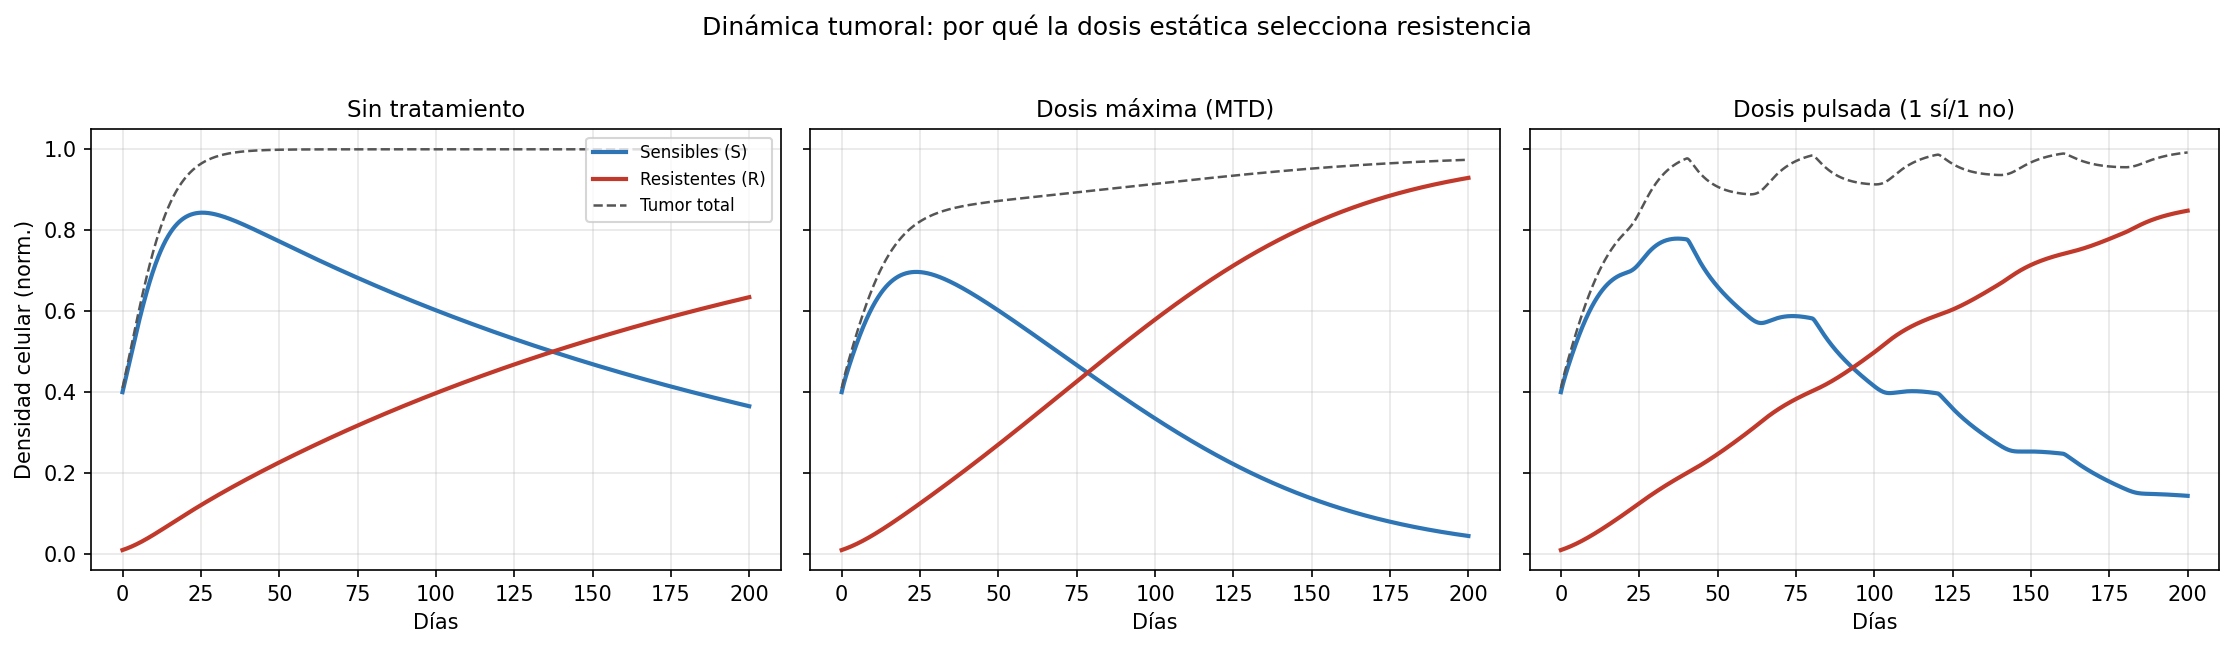
\includegraphics[width=0.85\textwidth]{images/dynamics_baseline.png}
\caption{Dinámica de referencia del simulador calibrado: evolución de las poblaciones sensible y resistente bajo distintos regímenes de dosificación.}
\label{fig:dynamics}
\end{figure}

\section{Validación del entorno y convergencia del aprendizaje}
\label{sec:res-aprendizaje}

Siguiendo la estrategia de validación incremental, se entrenó primero un agente único con PPO contra un tumor de comportamiento fijo. El retorno del agente de terapia mejoró de forma sostenida durante el entrenamiento, confirmando que el entorno es aprendible antes de introducir la complejidad multiagente.

Posteriormente, el entrenamiento adversarial por \emph{self-play} con MAPPO mostró la co-evolución de ambos agentes, como ilustra la Figura~\ref{fig:learning}. El régimen determinista garantiza que una misma semilla sea reproducible; no implica que todas las semillas converjan al mismo equilibrio. De hecho, la variabilidad entre inicializaciones es una limitación que se reporta explícitamente.

\begin{figure}[H]
\centering
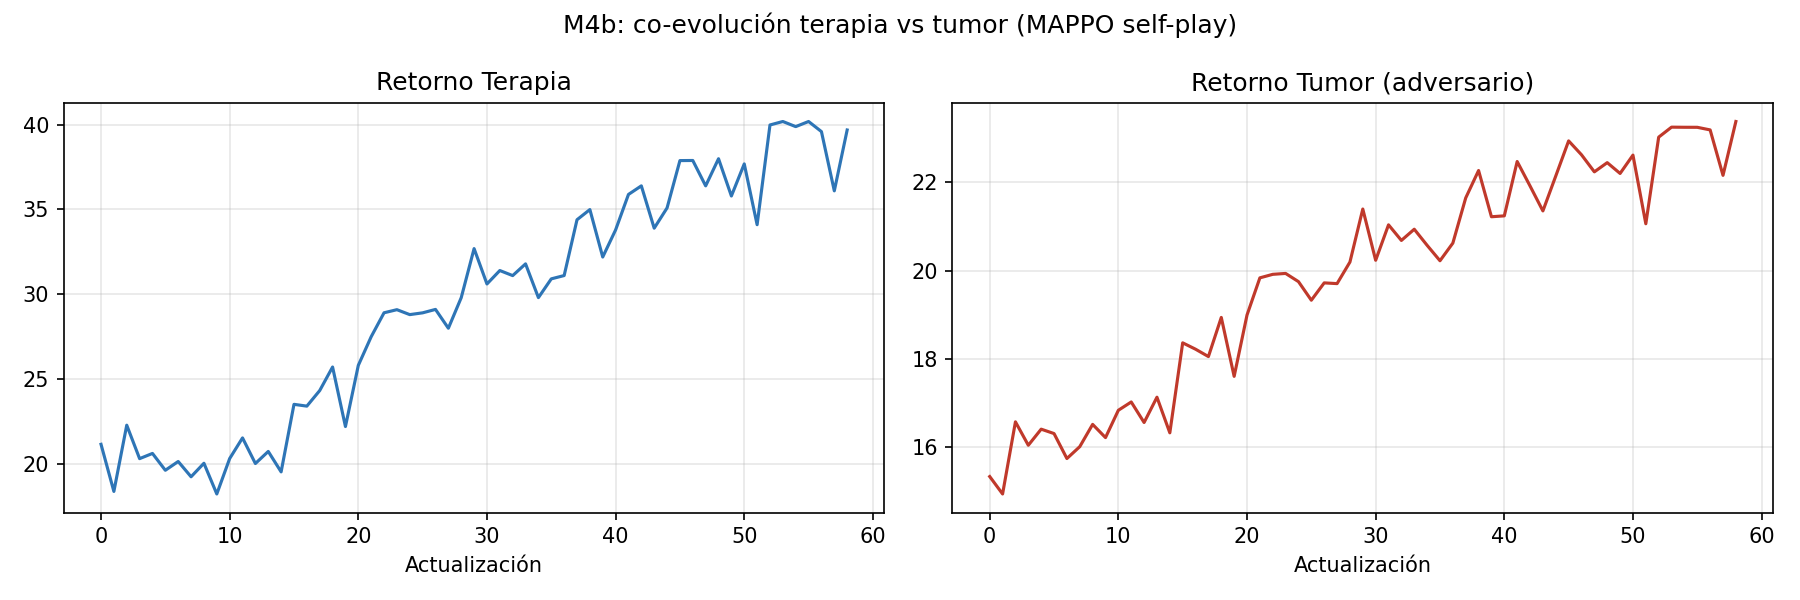
\includegraphics[width=0.95\textwidth]{images/mappo_learning_curves.png}
\caption{Curvas de aprendizaje del entrenamiento adversarial MAPPO por self-play: retorno del agente de terapia (izquierda) y del agente tumoral (derecha) a lo largo de las actualizaciones.}
\label{fig:learning}
\end{figure}

\section{Comparación frente a las líneas base}
\label{sec:res-comparacion}

La política aprendida se comparó contra tres referencias deterministas bajo la métrica de tiempo a falla combinado (TTP-combinado), reportando el modo de falla de cada estrategia. La Tabla~\ref{tab:res-baselines} resume los resultados de una evaluación representativa.

\begin{table}[H]
\centering
\caption{Comparación de estrategias bajo la métrica TTP-combinado, con el modo de falla. Métrica auditada mediante el procedimiento de diagnóstico.}
\label{tab:res-baselines}
\renewcommand{\arraystretch}{1.25}
\begin{tabular}{l|c|c|c|l}
\textbf{Estrategia} & \textbf{TTP (días)} & \textbf{Carga final} & \textbf{Frac.\ R final} & \textbf{Modo de falla} \\
\hline
Sin tratamiento     & 12  & 0.80 & 0.12 & carga progresó \\
MTD (dosis máx.)    & 13  & 0.09 & 0.52 & resistencia mayoría \\
Gatenby (adaptativa)& 27  & 0.38 & 0.53 & resistencia mayoría \\
MAPPO (aprendida)   & 41  & 0.79 & 0.51 & resistencia mayoría \\
\end{tabular}
\end{table}

Dos observaciones se desprenden de la Tabla~\ref{tab:res-baselines}. Primero, la métrica auditada revela que la ausencia de tratamiento falla por progresión de carga (día 12) mientras la fracción resistente permanece baja (0.12); todas las estrategias que tratan fallan, en cambio, por mayoría resistente. Segundo, la dosis máxima reduce la carga al mínimo (0.09) pero falla casi tan rápido como la ausencia de tratamiento (día 13), confirmando que la reducción agresiva del tumor precipita la resistencia. La política aprendida por MAPPO alcanza el mayor tiempo de manejo (41 días en esta corrida), superando a la heurística de Gatenby (27 días) y a la dosis máxima (13 días). La Figura~\ref{fig:ttp} muestra las trayectorias de carga tumoral y de fracción resistente para las cuatro estrategias.

\begin{figure}[H]
\centering
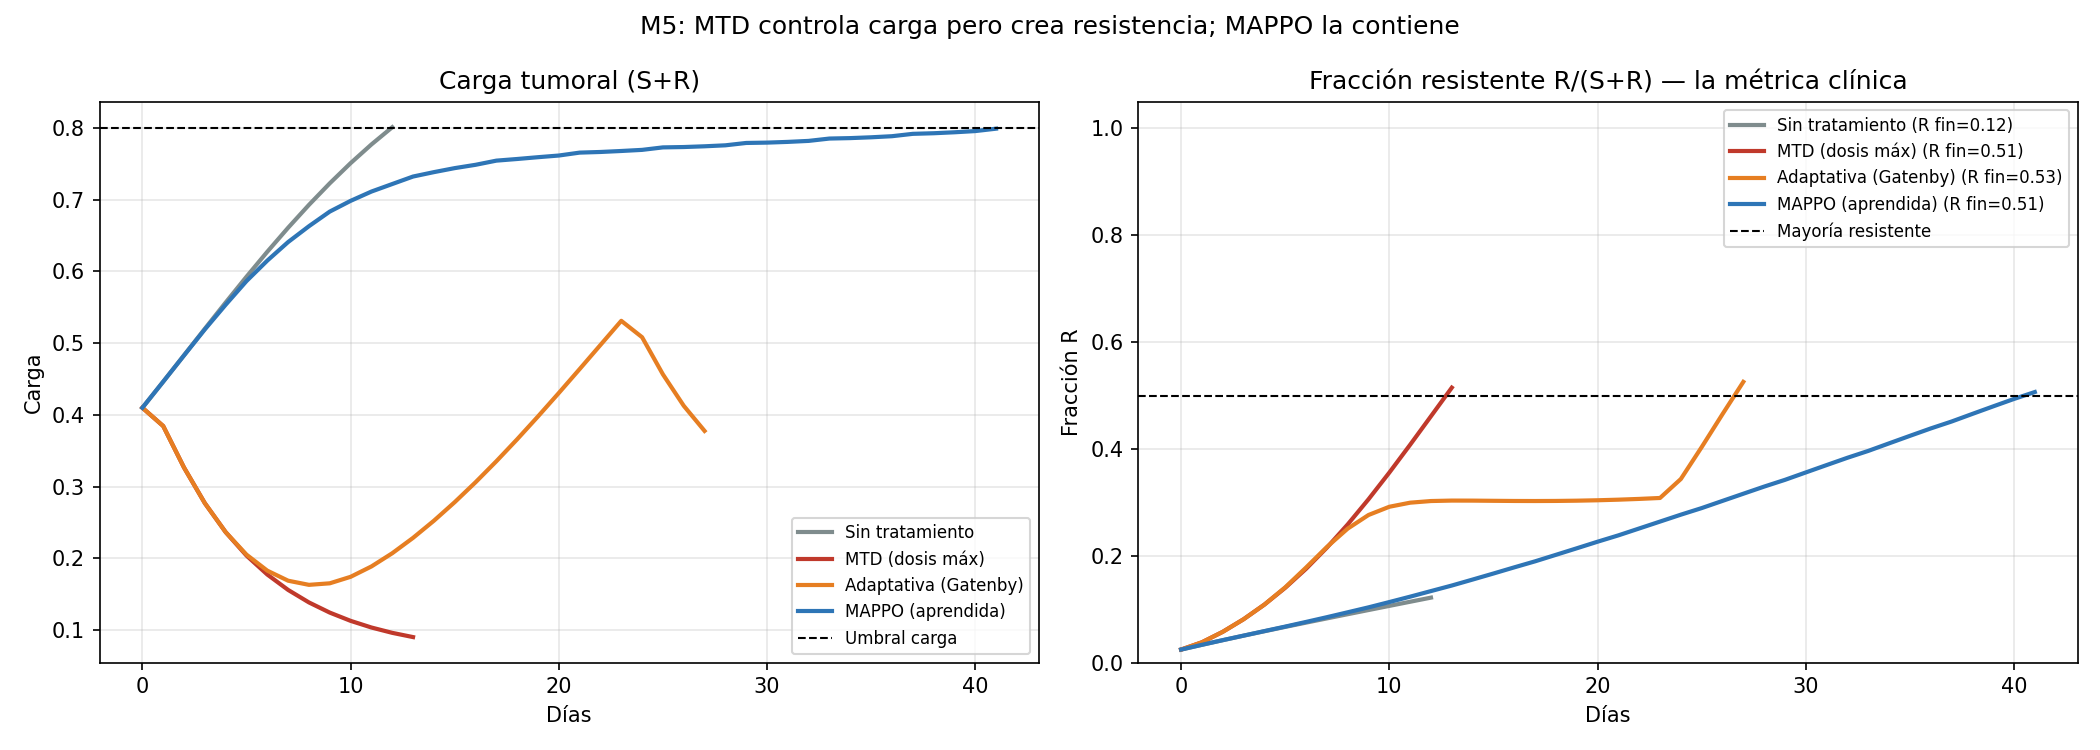
\includegraphics[width=0.95\textwidth]{images/evaluation_ttp.png}
\caption{Trayectorias de carga tumoral (izquierda) y de fracción resistente (derecha) para las cuatro estrategias. La dosis máxima controla la carga pero lleva la resistencia a su totalidad; la política aprendida retrasa la dominancia resistente.}
\label{fig:ttp}
\end{figure}

\subsection{Validación histórica multi-semilla y bimodalidad}

La corrida histórica del protocolo se evaluó sobre 15 semillas independientes. La distribución de los tiempos de manejo fue reportada como \textbf{bimodal}: una fracción de las corridas convergió a una cuenca con tiempos en el rango de 25 a 33 días, mientras que otra alcanzó una cuenca superior, en torno a los 41 días. Estas cifras pertenecen a una configuración anterior y no fueron revalidadas en la auditoría calibrada del 8 de septiembre de 2026; se conservan aquí como referencia metodológica, no como evidencia nueva.

Las afirmaciones de significancia de esta corrida histórica no deben transferirse automáticamente a la auditoría actual. La comparación calibrada nueva, con quince pares, se reporta en la Sección~\ref{sec:res-confirmacion}. La Figura~\ref{fig:validation} corresponde a la corrida histórica.

\begin{table}[H]
\centering
\caption{Validación histórica multi-semilla ($n=15$) del TTP-combinado. Las líneas base son deterministas. Esta tabla no corresponde a la auditoría calibrada del 8 de septiembre de 2026.}
\label{tab:res-multisemilla}
\renewcommand{\arraystretch}{1.25}
\begin{tabular}{l|c|c}
\textbf{Estrategia} & \textbf{TTP (días)} & \textbf{Significancia} \\
\hline
MTD (dosis máx.)     & 13                       & --- \\
Gatenby (adaptativa) & 27                       & --- \\
MAPPO (mejor corrida)& 41                       & --- \\
MAPPO (media, $n=15$)& $33{,}5 \pm 5{,}8$ (mediana 32) & $p<0{,}001$ vs.\ MTD y Gatenby \\
\end{tabular}
\end{table}

\begin{figure}[H]
\centering
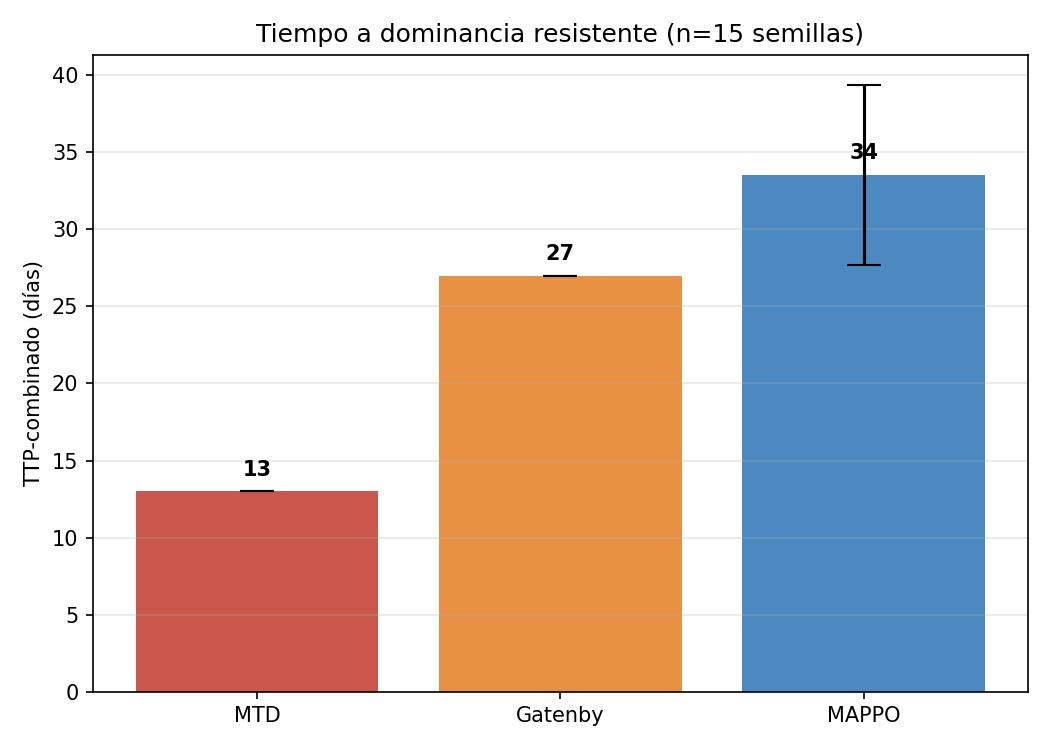
\includegraphics[width=0.6\textwidth]{images/validation_seeds.png}
\caption{Validación multi-semilla del TTP-combinado ($n=15$). La política aprendida supera a ambas líneas base deterministas; la barra de error refleja la dispersión bimodal del self-play.}
\label{fig:validation}
\end{figure}

\section{Mecanismo de la política aprendida}
\label{sec:res-mecanismo}

La inspección de las políticas de la cuenca superior revela el mecanismo descubierto por el agente. La Figura~\ref{fig:mecanismo} muestra que la política aplica una \textbf{dosificación pulsada e intermitente}: tras un periodo inicial, la dosis oscila entre valores bajos y nulos en lugar de mantenerse al máximo. Como consecuencia, la población sensible se mantiene en una densidad elevada que compite con la resistente y frena su expansión, mientras la fracción resistente crece lentamente hasta cruzar el umbral de mayoría. Este patrón corresponde al principio de la terapia adaptativa ---preservar una población sensible competidora--- redescubierto de forma autónoma por el agente, sin haber sido programado explícitamente.

\begin{figure}[H]
\centering
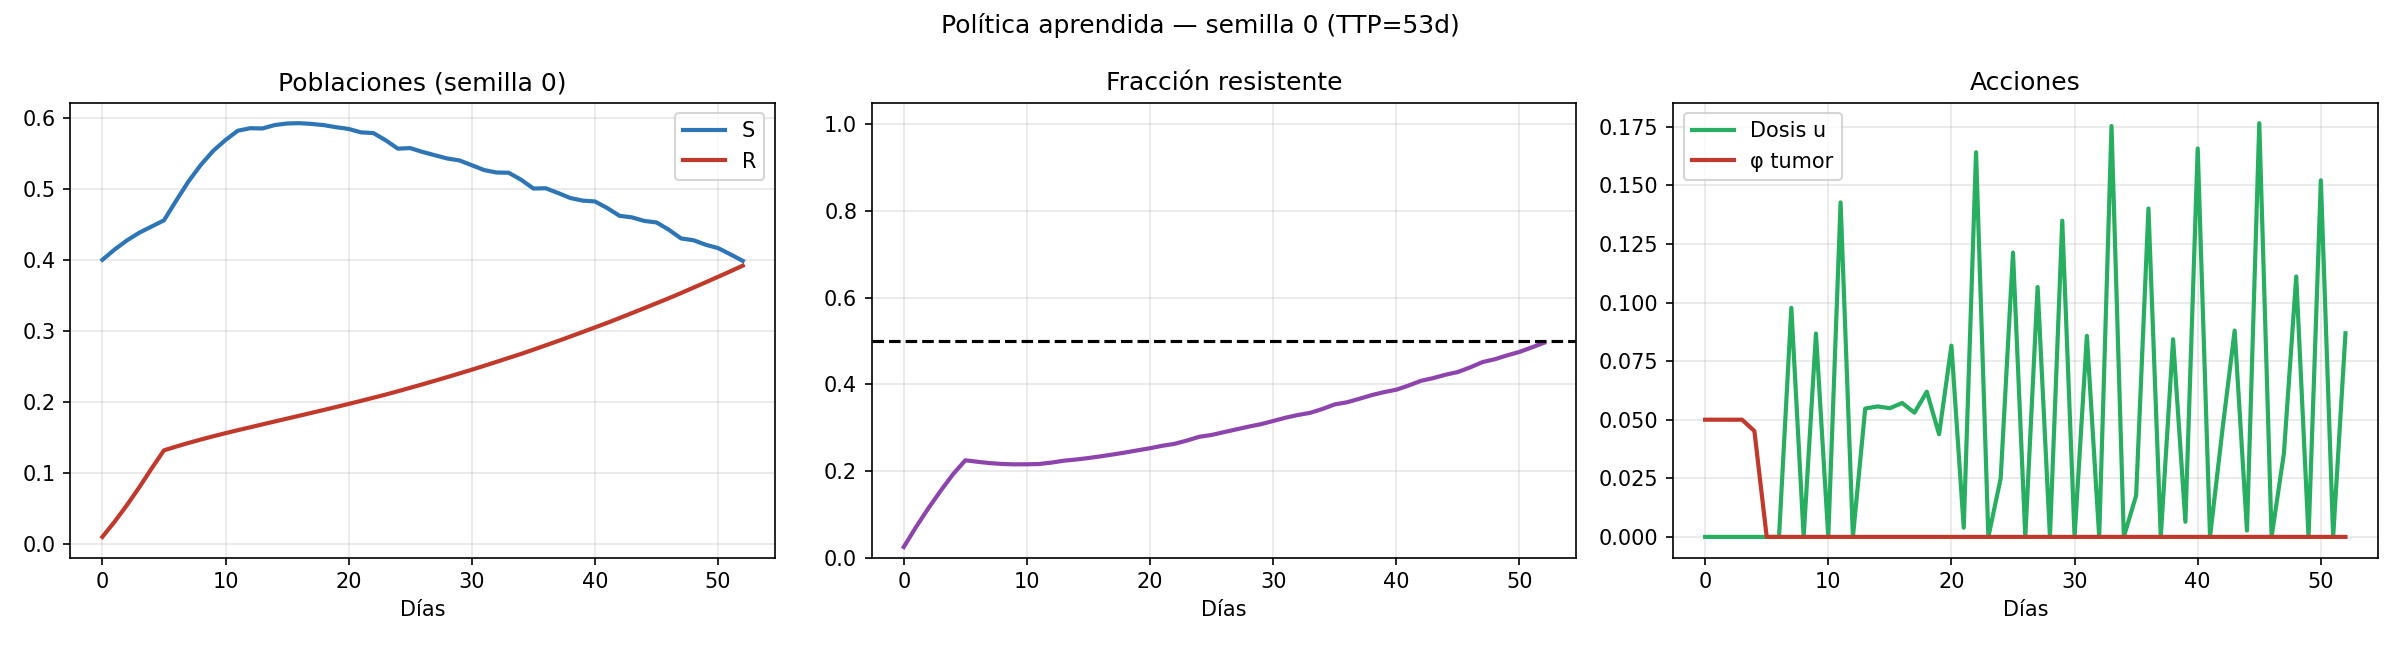
\includegraphics[width=0.95\textwidth]{images/policy_seed0.png}
\caption{Política aprendida de la cuenca superior: poblaciones (izquierda), fracción resistente (centro) y acciones de dosis y transición (derecha). La dosificación pulsada preserva la población sensible competidora.}
\label{fig:mecanismo}
\end{figure}

\section{Ablación del crítico centralizado (CTDE vs.\ IPPO)}
\label{sec:res-ablacion}

Para aislar la contribución del crítico centralizado, se comparó MAPPO (crítico condicionado al estado conjunto) con IPPO (crítico con observación local), manteniendo idénticos el actor, la observación de ejecución y todos los hiperparámetros. La verificación de la arquitectura confirmó que el cambio de variante modifica efectivamente la dimensión de entrada del crítico (3 para MAPPO, 2 para IPPO).

Bajo la métrica auditada y la calibración nueva, MAPPO alcanza una mediana de 34 días frente a 31 días de IPPO en quince pares de semillas (Tabla~\ref{tab:res-ablacion}). El contraste Wilcoxon pareado unilateral MAPPO$>$IPPO da $p=0{,}013759$; debe considerarse evidencia exploratoria condicionada al simulador. En esta corrida, las quince políticas IPPO fallaron por carga, mientras que MAPPO falló por resistencia en seis semillas y por carga en nueve.

\begin{table}[H]
\centering
\caption{Ablación calibrada del crítico centralizado ($n=15$). Ambas variantes comparten actor, observación de ejecución e hiperparámetros; solo difiere la entrada del crítico.}
\label{tab:res-ablacion}
\renewcommand{\arraystretch}{1.25}
\begin{tabular}{l|c|l}
\textbf{Variante} & \textbf{TTP (días)} & \textbf{Modo de falla} \\
\hline
MAPPO (crítico centralizado, CTDE) & $34$ [27,41] & 6 resistencia, 9 carga \\
IPPO (crítico local)               & $31$ [23,34] & 15 carga \\
\end{tabular}
\end{table}

\begin{figure}[H]
\centering
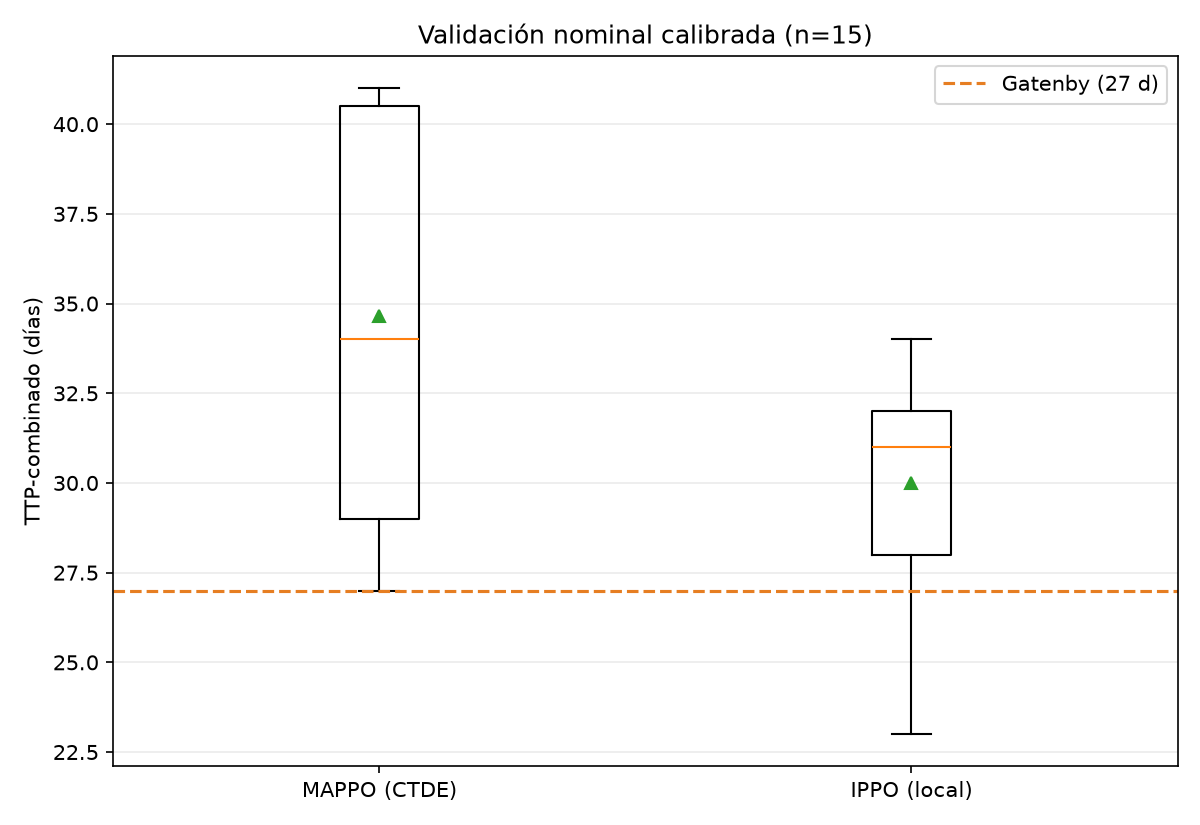
\includegraphics[width=0.6\textwidth]{images/ablation_ctde_15.png}
\caption{Ablación CTDE: MAPPO (crítico centralizado) frente a IPPO (crítico local) bajo el TTP-combinado.}
\label{fig:ablacion}
\end{figure}

\section{Análisis de sensibilidad}
\label{sec:res-sensibilidad}

En la auditoría calibrada se varió, una a la vez, cada una de las ocho constantes de dinámica y fármaco en factores de $0{,}8$ a $1{,}2$, manteniendo congeladas las políticas nominales. La Tabla~\ref{tab:res-sensibilidad} resume el rango del TTP-combinado de MAPPO sobre quince semillas. La política conserva una ventaja nominal en muchas perturbaciones, pero el ordenamiento $\text{MAPPO} > \text{Gatenby}$ no es universal: la reducción de $K$ y el aumento de $\mathrm{IC50}_S$ pueden eliminarla.

\begin{table}[H]
\centering
\caption{Análisis de sensibilidad calibrado. Rango del TTP-combinado de MAPPO sobre quince semillas al variar cada parámetro entre $0{,}8\times$ y $1{,}2\times$ su valor nominal.}
\label{tab:res-sensibilidad}
\renewcommand{\arraystretch}{1.25}
\begin{tabular}{l|c}
\textbf{Constante variada} & \textbf{MAPPO (rango, días)} \\
\hline
$\mathrm{IC50}_S$                  & 21--41 \\
$\mathrm{IC50}_R$                  & 27--41 \\
$\delta_S^{\max}$                 & 23--41 \\
$\delta_R^{\max}$                 & 26--41 \\
$\alpha_S$                         & 20--41 \\
$\alpha_R$                         & 26--45 \\
$\lambda_c$                        & 26--41 \\
$K$                                & 10--41 \\
\end{tabular}
\end{table}

El parámetro más sensible de esta corrida fue $K$: al reducirlo a $0{,}8K$, la mediana de MAPPO cayó a 25 días, frente a 34 días en el régimen nominal. También hubo degradación al aumentar $\mathrm{IC50}_S$ a $1{,}2\times$ (24 días) y $\alpha_S$ a $1{,}2\times$ (26 días). La Figura~\ref{fig:sensibilidad} muestra el barrido calibrado actualizado; los valores completos se conservan en el reporte de EXP-1.

\begin{figure}[H]
\centering
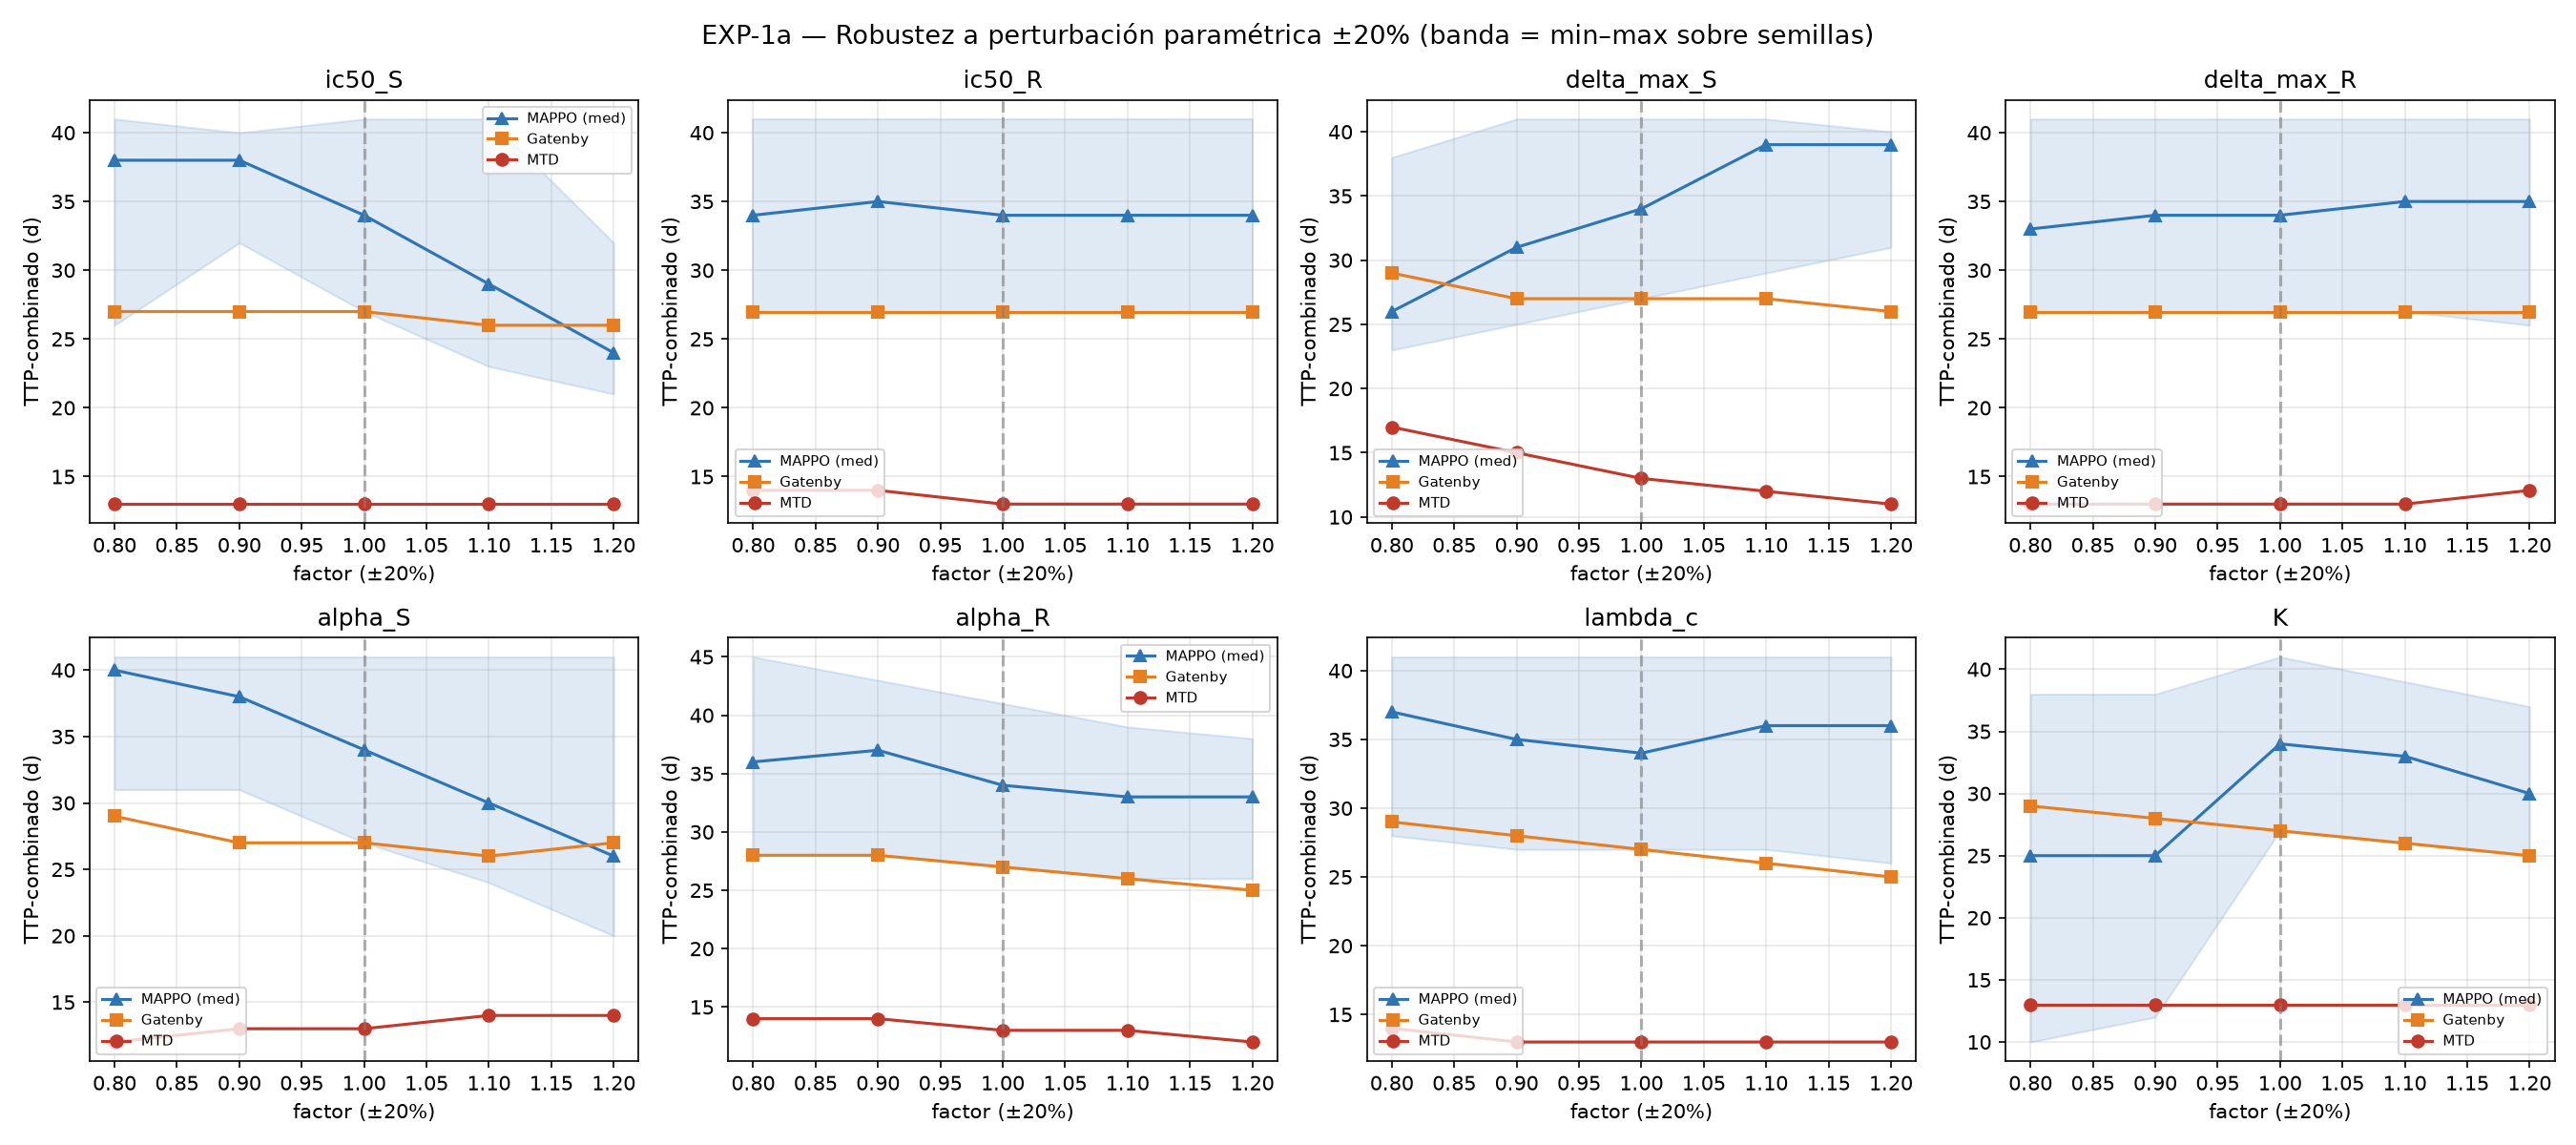
\includegraphics[width=0.95\textwidth]{images/exp1a_perturbacion_v2.png}
\caption{Análisis de sensibilidad calibrado de EXP-1. Cada panel muestra la mediana y la banda mínimo--máximo del TTP-combinado de MAPPO sobre quince semillas, junto con MTD y Gatenby, al variar una constante entre $0{,}8\times$ y $1{,}2\times$.}
\label{fig:sensibilidad}
\end{figure}

\section{Confirmación con la corrida completa reproducible}
\label{sec:res-confirmacion}

Para verificar que los hallazgos no dependen de la maquinaria de cómputo, se reejecutó la comparación nominal con el arnés reanudable y checkpointing intra-corrida descrito en la Sección~\ref{sec:checkpointing}. MAPPO e IPPO se entrenaron desde cero con el mismo presupuesto solicitado de \textbf{120\,000 pasos} (el último bloque produjo 120\,832 pasos), con \textbf{quince semillas independientes} por variante, usando la calibración real de DepMap/GDSC2. La evaluación se realizó con \texttt{TumorEnv} y $\phi=0{,}01$. Las líneas base, al ser deterministas, reprodujeron sus valores de forma exacta (sin tratamiento 12 días, MTD 13 días, Gatenby 27 días).

La Tabla~\ref{tab:res-confirmacion} reporta el resumen de las quince semillas; el detalle por semilla se conserva en el artefacto reproducible. La lectura principal es la \textbf{mediana}, el rango, los modos de falla y la tasa de éxito. MAPPO-CTDE alcanza 34 días [27--41] y supera a Gatenby en 13/15 semillas; IPPO alcanza 31 días [23--34] y lo hace en 12/15. El contraste Wilcoxon pareado unilateral MAPPO$>$IPPO da $p=0{,}013759$; se interpreta como evidencia exploratoria del simulador, no como eficacia clínica. El orden de medianas $\text{MAPPO} > \text{IPPO} > \text{Gatenby} > \text{MTD} > \text{Sin tratar}$ se observa en esta corrida.

\begin{table}[H]
\centering
\caption{Corrida calibrada reproducible (presupuesto solicitado de 120\,000 pasos; 120\,832 pasos efectivos; $n=15$ semillas por variante). TTP-combinado, modos de falla y tasa de éxito frente a Gatenby (27 días).}
\label{tab:res-confirmacion}
\renewcommand{\arraystretch}{1.25}
\resizebox{\textwidth}{!}{%
\begin{tabular}{l|c|l|c}
\textbf{Variante} & \textbf{TTP mediana [min,max]} & \textbf{Modo de falla} & \textbf{Éxito $>$Gatenby} \\
\hline
MAPPO (CTDE) & \textbf{34 [27,41]} & 6 resistencia, 9 carga & \textbf{13/15} \\
IPPO (local) & \textbf{31 [23,34]} & 15 carga & 12/15 \\
\end{tabular}
}
\end{table}

En la corrida actual, las dosis medias fueron aproximadamente 0.056 para MAPPO y 0.064 para IPPO. Este patrón es compatible con dosificación de baja intensidad, pero no basta por sí solo para afirmar un mecanismo clínico. El detalle por semilla y los checkpoints están en el reporte reproducible del repositorio; la figura calibrada se muestra a continuación.

\begin{figure}[H]
\centering
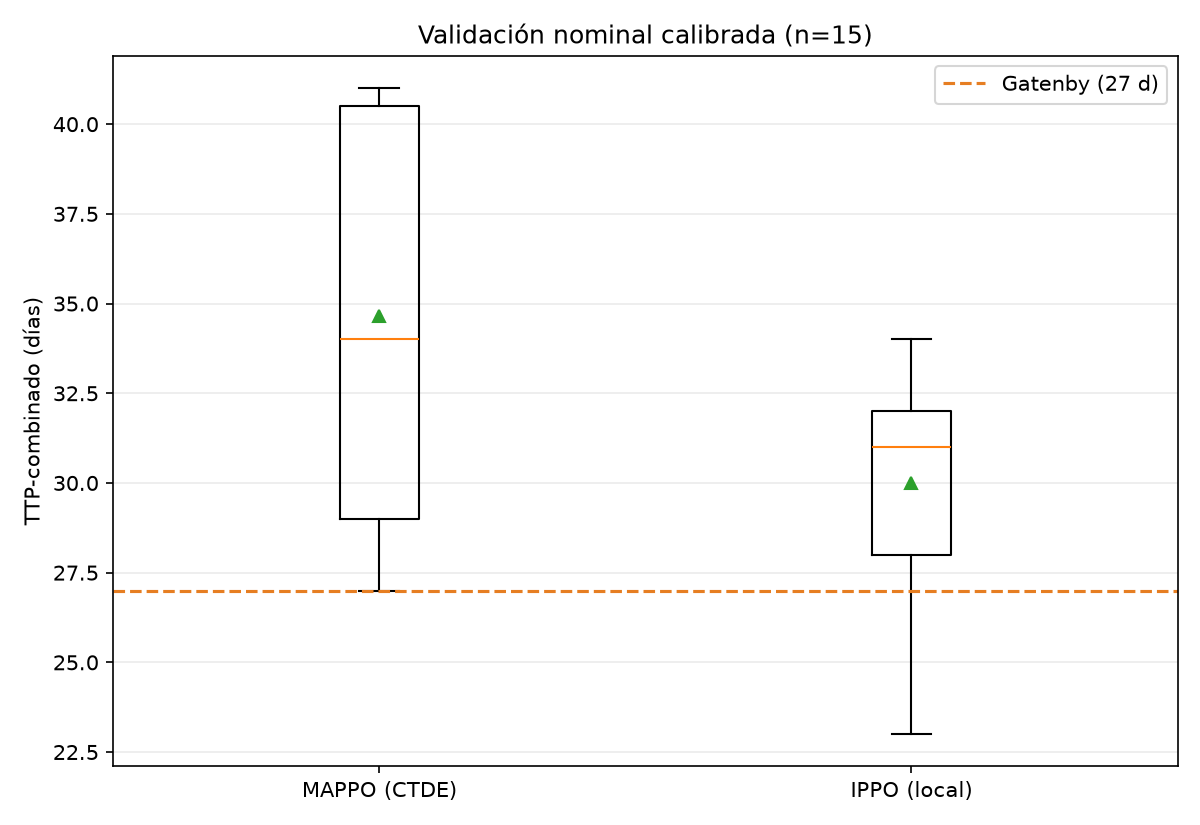
\includegraphics[width=0.72\textwidth]{images/validacion_calibrada_15semillas.png}
\caption{Validación nominal calibrada con quince semillas. La línea discontinua indica el TTP determinista de Gatenby (27 días); los puntos medios muestran la media de cada distribución.}
\label{fig:validation-calibrated}
\end{figure}

\subsection{Control de censura con horizonte extendido}

Para verificar que los tiempos reportados no fueran simplemente un tope impuesto por el
horizonte administrativo, se repitió la evaluación representativa con un horizonte de
360 días, conservando la calibración real, el adversario fijo y el TTP-combinado. Los
episodios sin tratamiento, MTD, Gatenby y MAPPO terminaron por carga o resistencia en
12, 13, 27 y 41 días, respectivamente. Ninguno alcanzó el día 360: los resultados son
fallos observados y no observaciones censuradas por el horizonte.

\subsection{EXP-2: adversario tumoral fortalecido}
\label{sec:res-exp2}

El segundo experimento examinó si la comparación MAPPO--IPPO se mantiene cuando el
agente tumoral dispone de un rango de acción mayor. Se evaluaron tres regímenes,
$\phi_{max}\in\{0{,}05,0{,}10,0{,}20\}$, con quince semillas por método y régimen
(90 celdas de 120\,000 pasos). Cada política se enfrentó al tumor adaptativo
co-entrenado de su propia celda; Gatenby se evaluó contra ese mismo tumor. Por tanto,
la prueba mide robustez frente a un adversario endógeno comparable, no una cota
matemática del peor caso.

La Tabla~\ref{tab:res-exp2} resume la corrida completa. MAPPO supera a IPPO con el
adversario nominal ($\phi_{max}=0{,}05$), pero la diferencia desaparece al ampliar el
rango de acción tumoral. La lectura es importante: la ventaja de CTDE es dependiente
del régimen y no debe presentarse como una propiedad universal del método.

\begin{table}[H]
\centering
\caption{EXP-2 calibrado: TTP-combinado frente al tumor adaptativo co-entrenado,
mediana [mín, máx], quince semillas por celda. Los valores $p$ son Wilcoxon pareado
unilateral MAPPO$>$IPPO, con corrección de Holm entre los tres regímenes.}
\label{tab:res-exp2}
\renewcommand{\arraystretch}{1.2}
\resizebox{\textwidth}{!}{%
\begin{tabular}{c|c|c|c|c|c|c}
\textbf{$\phi_{max}$} & \textbf{MAPPO} & \textbf{IPPO} & \textbf{$p$} & \textbf{Holm $p$} & \textbf{Éxito M} & \textbf{Éxito I} \\
\hline
0,05 & \textbf{44 [24,58]} & 29 [26,37] & 0,005 & 0,014 & 15/15 & 13/15 \\
0,10 & 28 [22,47] & 27 [23,35] & 0,648 & 0,648 & 15/15 & 14/15 \\
0,20 & 24 [21,50] & 26 [20,34] & 0,265 & 0,530 & 15/15 & 15/15 \\
\end{tabular}}
\end{table}

El modo de falla de MAPPO fue carga en 11/15, 15/15 y 13/15 semillas para los tres
regímenes, respectivamente, y resistencia en las restantes. IPPO terminó por carga
en las 45 semillas. Esto muestra además que fortalecer al adversario cambia no solo
el TTP, sino también qué límite del sistema se alcanza primero. Los resultados son
evidencia in silico de sensibilidad al régimen adversarial; no implican eficacia
clínica ni permiten afirmar que un adversario aprendido sea óptimo.

\begin{figure}[H]
\centering
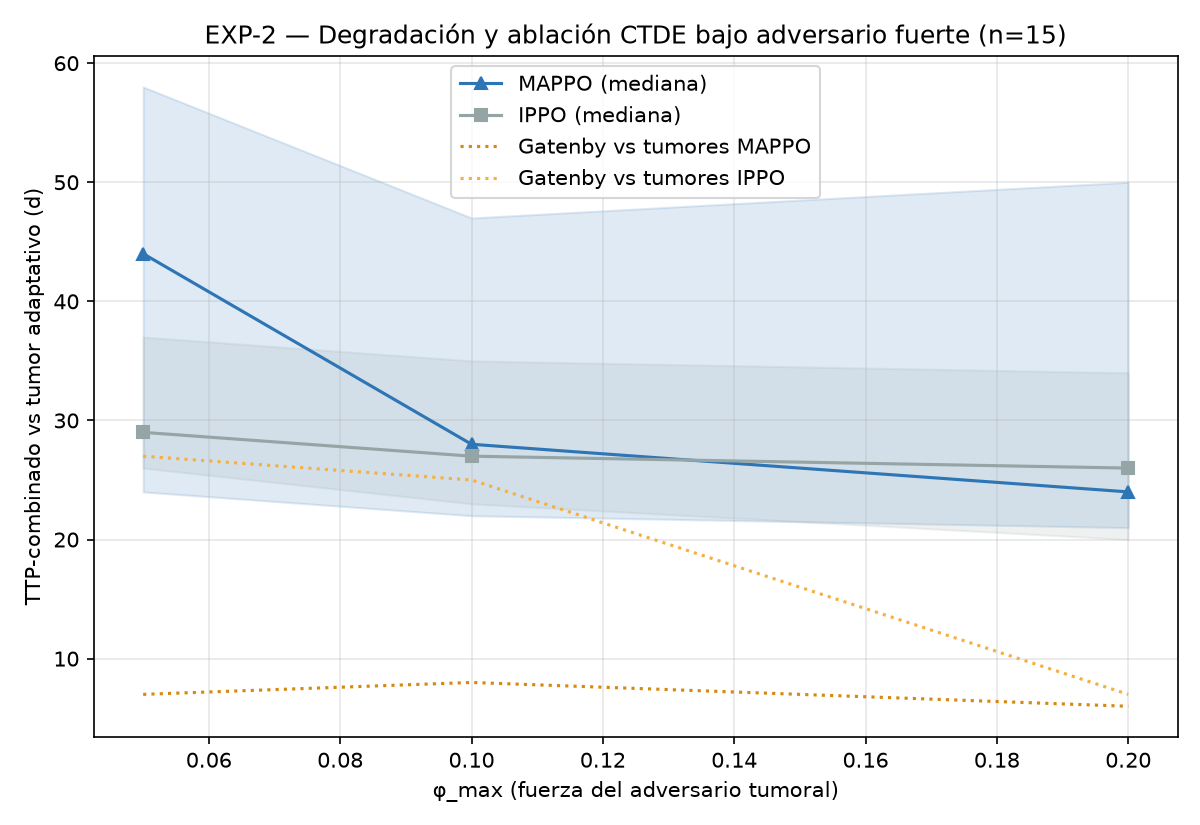
\includegraphics[width=0.78\textwidth]{images/exp2_adversario_v2.png}
\caption{EXP-2 calibrado. La mediana y el rango del TTP-combinado de MAPPO e IPPO
se muestran al aumentar el límite de transición tumoral $\phi_{max}$.}
\label{fig:exp2-adversario}
\end{figure}

\section{Robustez adversarial mediante explotabilidad}
\label{sec:res-explotabilidad}

Un juego resuelto por \textit{self-play} puede sobreajustarse al adversario con el que
co-evolucionó. Para examinar esta posibilidad se evaluó la \textbf{explotabilidad} de
cada política, siguiendo el estándar de la teoría de juegos computacional~\cite{deWitt2020}.
Se congeló cada terapia, se entrenaron cinco adversarios tumorales dedicados desde
reinicios independientes y se conservó el más dañino. La corrida titular usó quince
semillas, $\phi_{max}=0{,}05$ y 120\,000 pasos. La explotabilidad se define como
$\text{TTP}_{self-play}-\text{TTP}_{best-response}$; una brecha menor indica menor
degradación ante el atacante dedicado. PPO no garantiza el óptimo global, por lo que
estos resultados son una estimación empírica y no una cota matemática del peor caso.

\begin{table}[H]
\centering
\caption{Benchmark V2 calibrado ($n=15$ semillas, cinco reinicios de \textit{best-response}). Se reporta la mediana [mín, máx] del TTP-combinado frente al tumor de \textit{self-play}, frente al mejor atacante dedicado y la brecha de explotabilidad. Gatenby, sometido a cinco reinicios análogos, obtuvo 7 días.}
\label{tab:res-explotabilidad}
\renewcommand{\arraystretch}{1.25}
\resizebox{\textwidth}{!}{%
\begin{tabular}{l|c|c|c|c}
\textbf{Variante} & \textbf{TTP self-play} & \textbf{TTP best-response} & \textbf{Explotabilidad} & \textbf{TTP $>$ 7 d} \\
\hline
MAPPO (CTDE) & $44\ [24,58]$ & $\mathbf{14\ [11,14]}$ & $30\ [11,44]$ & 15/15 \\
IPPO (local) & $29\ [26,37]$ & $11\ [10,12]$          & $18\ [14,27]$ & 15/15 \\
\end{tabular}
}%
\end{table}

La terapia MAPPO conserva un TTP absoluto mayor frente al mejor atacante encontrado
(14 frente a 11 días), pero también presenta una brecha puntual mayor (30 frente a
18 días). El contraste unilateral preespecificado para la hipótesis
$\text{explotabilidad}_{MAPPO}<\text{explotabilidad}_{IPPO}$ no respalda esa dirección
($p=0{,}993$); por tanto, no se afirma que MAPPO sea menos explotable. El resultado sí
obliga a separar dos ideas: un TTP absoluto más alto no equivale automáticamente a una
menor sensibilidad a un atacante dedicado.

El cross-play aporta una prueba fuera del compañero de entrenamiento: MAPPO frente a
la población de tumores IPPO obtuvo 35 días [24,41], mientras IPPO frente a tumores
MAPPO obtuvo 27 días [12,29]. La asimetría sugiere mejor transferencia de MAPPO en
este escenario, aunque no constituye por sí sola una prueba de significancia ni de
robustez universal.

\begin{figure}[H]
\centering
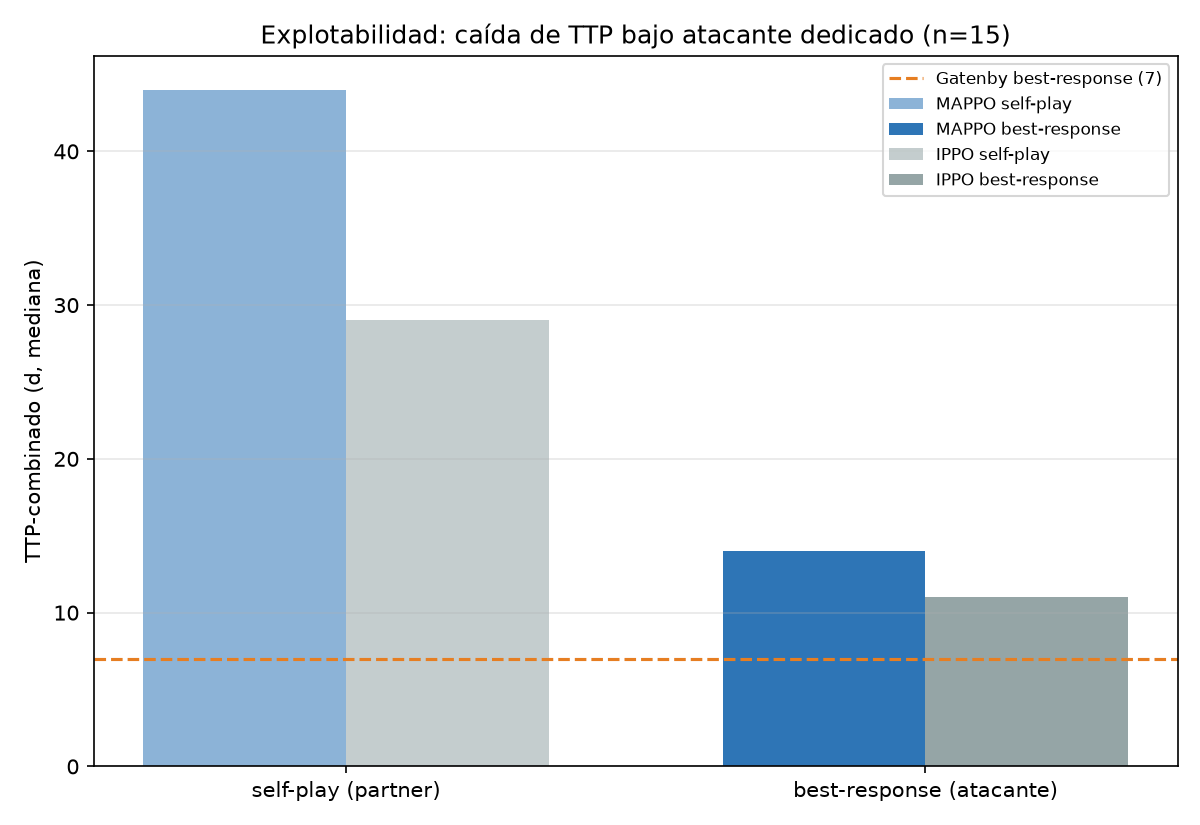
\includegraphics[width=0.7\textwidth]{images/benchmark_exploit_v2.png}
\caption{Benchmark V2: TTP-combinado de self-play y frente al mejor atacante dedicado
para MAPPO e IPPO. La línea de Gatenby corresponde a su propia best-response aproximada.}
\label{fig:explotabilidad}
\end{figure}

En conjunto, la auditoría calibrada muestra que la política aprendida extiende el tiempo
de manejo simulado frente a MTD y Gatenby en el escenario nominal, con una ventaja de
MAPPO sobre IPPO en la comparación nominal y en cross-play. EXP-2 muestra, sin embargo,
que esa ventaja desaparece al fortalecer el adversario; el benchmark V2 muestra además
que el TTP absoluto y la explotabilidad son propiedades distintas. Por tanto, el
resultado debe interpretarse como evidencia \textit{in silico} de comportamiento
adaptativo bajo el modelo especificado, no como eficacia clínica ni como robustez
universal.
